\subsection{Markov Processes}

\newcommand{\Models}{|\!\!\!\equiv}

Concurrent systems are often modeled by a state transition system, such as Kripke structure, where uncertainties in the state transitions are captured by nondeterministic choices of the next state. Replacing the nondeterminism in the state transitions with state transition probabilities, the structure can be modeled by Markov chains. A Continuous Time Markov Chain (CTMC) comprises a set of states and an infinitesimal generator matrix, representing the rate of the state transition between two states. Similarly, a Discrete Time Markov Chain (DTMC) comprises a set of states and a probability transition matrix, representing the probability of the state transition between two states. 


Formally, Markov chains can be defined as a stochastic process and represented by a state transition diagram. Let $\mathcal{P}=\langle\Omega,F,P\rangle$ be a probability space, where $\Omega$ is a sample description space, $F\subseteq 2^\Omega$ is a sigma-algebra of events and $P:F\rightarrow[0,1]$ is a probability measure. A Random Variable (RV) $X:\Omega\rightarrow\mathbb{R}$ is a mapping from the sample description space to the real line such that the set $\{\zeta\in\Omega:X(\zeta)\leq x\}$ is an event for every $x\in\mathbb{R}$. For Markov chains with a finite set of states $S=\{s_1,\ldots,s_n\}$, we can write a RV $X$ as a mapping $X:\Omega\rightarrow S$. With this representation, we write $P[X=s_i]$ for the probability $P(\{\zeta\in\Omega:X(\zeta)=s_i\})$. 
For a discrete RV $X:\Omega\rightarrow S$, the {\em Probability Mass Function} (PMF) of $X$ is a function $P_X:S\rightarrow[0,1]$ that associates a probability to each state $s\in S$ as $P_X(s)=P[X=s]$ such that $\sum_{s\in S} P_X(s)=1$.


A stochastic process $X:\mathbb{R}^+\rightarrow(\Omega\rightarrow\mathbb{R})$ is a mapping from the time to RVs. Additionally, a sample function $X:\Omega\rightarrow(\mathbb{R}^+\rightarrow\mathbb{R})$ is also called a stochastic process. A DTMC is a stochastic process $D:\mathbb{N}^+\rightarrow(\Omega\rightarrow S)$ that satisfies the memoryless property $P[D(k)=s_k|D(k-1)=s_{k-1},\ldots,D(0)=s_0]=P[D(k)=s_k|D(k-1)]$ for all $s_k,\ldots,s_0\in S$ and for all $k\in\mathbb{N}^+$. DTMCs can be represented by {\em State Transition Diagram} (STD) of $\langle S,\mathbf{M}\rangle$, where $S=\{s_1,\ldots,s_n\}$ is a set of states and $\mathbf{M}\in\mathbb{R}^{n\times n}$ is a probability transition matrix such that $\mathbf{M}_{ij}$ = $P[D(k+1)=s_i|D(k)=s_j]$ for $k\geq 0$. An STD $D$ is a labeled directed graph whose nodes are $S$ and whose labeled directed edges are $\{(s_j, s_i, \mathbf{M}_{ij})\in S\times S\times [0,1]: \mathbf{M}_{ij} > 0\}$.


In order to compute the fraction of paths that satisfy certain properties, an STD of a DTMC can be extended with an initial state and a function that maps each state with a set of atomic properties that are true in the state. Formally, the structure is a quadruple $\langle S, S_i, T, L\rangle$, where
\begin{itemize}
\item $S$ is a finite set of states
\item $S_i\in S$ is an initial state,
\item $T$ is a transition probability function, $T: S\times S \rightarrow [0,1]$ such that for all $s\in S$
$\sum_{s’\in S} T(s,s’) = 1$
\item $L$ is a labeling function assigning atomic propositions to states, i.e. $L: S->2^A$
\end{itemize}


A path from a state $s_0$ in a structure is an infinite sequence
$s_0 \rightarrow s_1 \rightarrow \cdots \rightarrow s_n \rightarrow\cdots$ of states. Given a structure and a state $s_0$, a probability measure $\mu_m$ can be defined on the set of paths starting from $s_0$. $\mu_m$ is defined on the probability space $\langle X, A\rangle$, where $X$ is the set of paths starting from $s_0$ and $A$ is a sigma-algebra on $X$ generated by sets $\{\sigma \in X: \sigma\uparrow n = s_0 \rightarrow\cdots\rightarrow s_n\}$ of paths with a common finite prefix $s_0\rightarrow\cdots\rightarrow s_n$.

The measure $\mu_m$ is defined as follows:
$\mu_m(\{\sigma \in X: \sigma\uparrow n = s_0 \rightarrow\cdots\rightarrow s_n\}) = 
T(s_0,s_1)\times\cdots\times T(s_{n-1},s_n)$ and $\mu_m(\{\sigma \in X: \sigma\uparrow 0 = s_0\}) = 1$. The measure $\mu_m$ defines the measure on all sets of paths in the sigma-algebra $A$.


Another research direction on Markov chains is to model statistical properties of a large scale system. In this approach, the state of a system as a whole is a Probability Mass Function (PMF), representing the portions of individual systems in a certain state and the computation paths are the trajectories of PMFs over time.

\begin{figure}
\centering
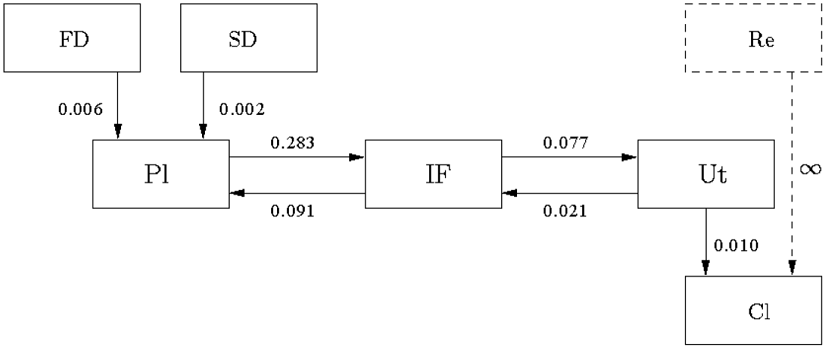
\includegraphics[width=.6\columnwidth]{assets/compartment_model.png}
\caption{
    A compartment model (CTMC), describing a drug ADME process: the boxes are the compartments representing Fast-acting Drug, Slow-acting Drug, Plasma, Interstitial Fluid, Site of Utilization, and Cleared respectively; and the numbers are the state transition rates. Re is an artificial state, where the drug is cleared instantly.}
\label{fig:comparment}
\end{figure}

For example, Fig.~\ref{fig:comparment} shows a compartment model for a drug Absorption, Distribution, Metabolism, and Excretion (ADME) process. Compartment models are a Markov chain that has been used in Pharmaceutics to describe drug kinetics. Using iLTL one can specify desirable properties such as a minimum toxic concentration, minimum effective concentration, conditions for multi-dosage regimen, etc. and find a prescription (the portions of drug in FD, SD, and Re at the initial state) that can satisfy the specification.



\subsection{Probabilistic real time CTL (PCTL)}
\label{sec:pctl}
\todo[inline]{move to Section 3 (Programming and Verification}

The set of PCTL formulas is divided into path formulas and state formulas. State formulas represent properties of states and path formulas represent properties of paths, sequences of states.
The syntax of PCTL is as follows
\begin{itemize}
\item Each atomic proposition $a\in A$ is a state formula, where $A$ is a finite set of atomic propositions.
\item If $f_1$ and $f_2$ are state formulas, then so are $\neg f_1$, $f_1 \wedge f_2$, $f_1 \vee f_2$, $f_1\rightarrow f_2$.
\item If $f_1$ and $f_2$ are state formulas and $t$ is a non-negative integer or $\infty$, then $f_1 U^{\leq t} f_2$ and $f_1 {\cal U}^{\leq t} f_2$ are path formulas
\item If $f$ is a path formula and $p$ is a real number with $0\leq p\leq 1$, then $[f]_{\geq p}$ and $[f]_{>p}$ are state formulas.
\end{itemize}
The propositional connectives $\neg$, $\vee$, $\wedge$ and $\rightarrow$ have their usual meanings. $U$ is the (strong) until operator, and $\cal U$ is the unless (or weak until) operator. Given a state $s$, the formula $[f]_{\geq p}$ and $[f]_{>p}$ mean that $f$ holds for a path starting from $s$ with a probability of at least $p$ and greater than $p$ respectively.

PCTL formulas are interpreted DTMCs. A specific initial state is associated the DTMC and for each state, there is an assignment of truth values to atomic propositions appearing in a given formula.

Formally, a structure is a quadruple $\langle S, S_i, T, L\rangle$, where $S$ is a fnite set of states, $s_i\in S$ is an initial state, $T$ is a transition probability function, $T: S\times S \rightarrow [0,1]$, such that for all $s \in S$, $\sum_{s'\in S} T(s,s') = 1$, $L:S\rightarrow 2^A$ is a labeling function assigning atomic propositions to states.

A path $\sigma$ from a state $s_0$ is an infinite sequence
$$s_0\rightarrow s_1\rightarrow \cdots \rightarrow s_n \rightarrow \cdots
$$
of states with $s_0$ at the first state. The $n^{th}$ state of $\sigma$ is denoted $\sigma[n]$ and the prefix of $\sigma$ of length $n$ is denoted $\sigma\uparrow n$, i.e.,
$$\sigma\uparrow n = s_0\rightarrow s_1\rightarrow \cdots \rightarrow s_n.
$$

For each state $s_0$, a probability measure $\mu_m$ is defined on the probability space $\langle X, A\rangle$, where $X$ is a set of paths starting from $s_0$ and $A$ is s sigma-algebra on $X$ generated by the sets
$$\{ \sigma\in X : \sigma\uparrow n = s_0\rightarrow \cdots \rightarrow s_n\}
$$
of paths with a common finite prefix. For each finite sequence $s_0\rightarrow s_1\rightarrow \cdots \rightarrow s_n$, the measure $\mu_m$ is 
$$\mu_m(\{ \sigma\in X : \sigma\uparrow n = s_0\rightarrow \cdots \rightarrow s_n\}) = T(s_0,s_1)\times\cdots\times T(s_{n-1},s_n)
$$
and when $n=$, $\mu_m(\{ \sigma\in X : \sigma\uparrow 0 = s_0\}) = 1$.

The truth value of a state formulas $f$ for a structure K can be defined by a satisfaction relation $s\models_K f$, meaning that the state formula $f$ is true in state $s$ and the truth value of a path formula $f$ can be defined by a satisfaction relation $\sigma \Models_K f$, meaning that the path $\sigma$ satisfies $f$. Formally, the satisfaction relations are defined as follows
\begin{eqnarray*}
s\models_K a &\Leftrightarrow& a \in L(s)\\
s\models_K\neg f &\Leftrightarrow& s \not\models_K f\\
s\models_K f_1 \wedge f_2 &\Leftrightarrow& s\models_K f_1\mbox{ and }s\models_K f_2\\
s\models_K f_1 \vee   f_2 &\Leftrightarrow& s\models_K f_1\mbox{ or }s\models_K f_2\\
s\models_K f_1\rightarrow f_2 &\Leftrightarrow& s\models_K\neg f_1\mbox{ or }s\models_K f_2\\
\sigma\Models_K f_1 U^{\leq t} f_2 &\Leftrightarrow& \parbox{8cm}{there exists an $i\leq t$ such that $\sigma[i]\models_K f_2$ and for all $j\in[0,\ldots,i)$, $\sigma[j]\models_K f_1$.}\\
\sigma\Models_K f_1 {\cal U}^{\leq t} f_2 &\Leftrightarrow& \parbox{8cm}{$\sigma\Models_K f_1 U^{\leq t} f_2$ or for all $j\in[0,\ldots,t]$, $\sigma[j]\models_K f_1$.}\\
s\models_K[f]_{\geq p} &\Leftrightarrow&\parbox{8cm}{the $\mu_m$ of the set of paths $\sigma$ starting in $s$ for which $\sigma\Models_K f$ is at least p.}\\
s\models_K[f]_{> p} &\Leftrightarrow&\parbox{8cm}{the $\mu_m$ of the set of paths $\sigma$ starting in $s$ for which $\sigma\Models_K f$ is greater than p.}
\end{eqnarray*}
Using the ternary satisfaction relations $\models_K f \Leftrightarrow s_i \models_K f$.

\subsection{iLTL}
\label{sec:itlt}
\todo[inline]{move to Section 3 (Programming and Verification}
